\chapter{Introduction}

\section{What is SQL?}
Structured Query Language or SQL is a common programming language for relational databases. Many IT professionals like data analysts, database administrators, SQL developers and data scientists often require using this coding language. Having knowledge and expertise in SQL is important for these roles.  SQL, can be defined as a database coding language that extracts and manages data stored in a relational database. A relational database means you store and retrieve data in the form of relations or tables. For example, a table contains information about employees, such as employee id, name, contact number and department. This employee table is a relational database with only one relation called employee. You use SQL to communicate with a database. Using different commands, SQL tells the database what to do.

You can use the SQL commands to update, search, retrieve, add and delete data. Some of the standard and widely used commands are: Select, Update, Create, Delete, Group By and Insert. Though SQL is a standard of the American National Standards Institute (ANSI) and the International Organisation for Standardisation (ISO), many organisations use proprietary extensions based on the database used by the organisation. Furthermore, like other programming languages, SQL has a markup. This makes it essential for IT professionals to learn SQL markup.

\section{Constraints in SQL}
SQL constraints are used to specify rules for the data in a table.

Constraints are used to limit the type of data that can go into a table. This ensures the accuracy and reliability of the data in the table. If there is any violation between the constraint and the data action, the action is aborted.

Constraints can be column level or table level. Column level constraints apply to a column, and table level constraints apply to the whole table.

The following constraints are commonly used in SQL:
\begin{itemize}
	\tightlist
	\item \textbf{NOT NULL} - Ensures that a column cannot have a NULL value
	\item \textbf{UNIQUE} - Ensures that all values in a column are different
	\item \textbf{PRIMARY KEY} - A combination of a NOT NULL and UNIQUE. Uniquely identifies each row in a table
	\item \textbf{FOREIGN KEY} - Prevents actions that would destroy links between tables
	\item \textbf{CHECK} - Ensures that the values in a column satisfies a specific condition
	\item \textbf{DEFAULT} - Sets a default value for a column if no value is specified
	\item \textbf{CREATE INDEX} - Used to create and retrieve data from the database very quick.
\end{itemize}

\section{SQL Commands}
\begin{figure}[h]
	\centering
	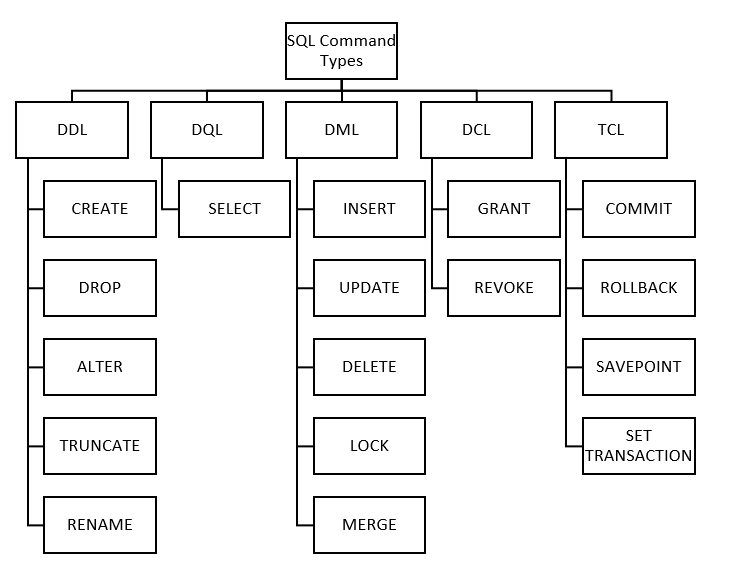
\includegraphics[width=0.85\linewidth]{img/a1}
	\caption{\textit{Various SQL Commands}}
	\label{fig:sql_commands}
\end{figure}


\chapter{DDL in MySQL}
\section{Introduction}
DDL is the short name for Data Definition Language, which deals with database schemas and descriptions of how the data should reside in the database. MySQL DDL is a subgroup of SQL commands among four: DDL, DML, DCL, and TCL. Structured Query Language(SQL) is the primary language of a database which performs different operations and queries in the available MySQL database, including creating a database or table to drop the same and others like updating, inserting, etc. The MySQL DDL gets involved with the schemas and explanations of the database to display how the database data should exist on the server. The DDL commands are significant for expressing and altering the structure of database tables, schemas or objects.

Various DDL Commands:
\begin{itemize}
	\tightlist
	\item \textbf{CREATE} - to create a database and its objects like (table)
	\item \textbf{ALTER} - alters the structure of the existing database
	\item \textbf{DROP} - delete objects from the database
	\item \textbf{TRUNCATE} - remove all records from a table, including all spaces allocated for the records that are removed
	\item \textbf{COMMENT} - add comments to the data dictionary
	\item \textbf{RENAME} - rename an object	
\end{itemize}

\section{CREATE Command}
The CREATE statement is written using the following syntax:
\begin{lstlisting}[language=sql]
	CREATE DATABASE DatabaseName;
	CREATE TABLE TableName 
	(Column1 Datatype1, 
	Column2 Datatype2,
	…
	ColumnNDatatypeN);
\end{lstlisting}

For Example, we will create a table named ‘Emp’ with some fields and similar data types that are valid in MySQL and, respectively a database named ‘EmpDB’ in MySQL server using the queries below:
\begin{lstlisting}[language=sql]
	CREATE DATABASE EmpDB;
	CREATE TABLE Emp 
	(Emp_ID INT PRIMARY KEY,
	 Emp_Name VARCHAR(255), 
	 Emp_City VARCHAR(255), 
	 Emp_AdmDate DATE NOT NULL);
\end{lstlisting}

\section{ALTER Commande}
ALTER DDL command is applied to modify the structure of the present database and related tables.
With Alter query, we can add, alter or delete the present constraints on a table or columns on the table. 
The syntax is mentioned below:
\begin{lstlisting}[language=sql]
	ALTER TABLE TableName ADD ColumnNameData_Type;
	ALTER TABLE TableName DROPColumnName;
	ALTER TABLE TableName MODIFY COLUMNColumnNameData_Type;	
\end{lstlisting}
Example:
\begin{lstlisting}[language=sql]
	ALTER TABLE Emp ADD Emp_Contact INT NOT NULL;
	ALTER TABLE Emp DROP Emp_Contact;
	ALTER TABLE Emp MODIFY COLUMN Emp_AdmDate Year;	
\end{lstlisting}

\section{DROP Command}
This MySQL command is used to remove the database objects. In simple words, to delete the table existing in your database using the drop query syntax:
\begin{lstlisting}[language=sql]
	DROP TABLE TableName;
\end{lstlisting}
Example:
\begin{lstlisting}[language=sql]
	DROP TABLE Emp;
\end{lstlisting}

\section{TRUNCATE Command}
The truncate DDL command is implemented to delete all the data rows from the database table, which includes removing all spaces assigned for those table records.

The syntax of the TRUNCATE command is identical to the DROP statement as follows:
\begin{lstlisting}[language=sql]
	TRUNCATE TABLE TableName;
\end{lstlisting}
Example:
\begin{lstlisting}[language=sql]
	TRUNCATE TABLE Emp;
\end{lstlisting}

\section{RENAME Command}
The Rename DDL command query allows renaming any database objects in the server if needed for any admin works. Sometimes we want to modify the present table name and rename it. For this, let us apply the succeeding syntax with ALTER DDL command:
\begin{lstlisting}[language=sql]
	ALTER TABLE TableName_A RENAME TO TableName_B;
\end{lstlisting}
Example:
\begin{lstlisting}[language=sql]
	ALTER TABLE Emp RENAME TO Emp_Data;
\end{lstlisting}


\chapter{DML in MySQL}
\section{Introduction}
DML is short name of Data Manipulation Language which deals with data manipulation and includes most common SQL statements such SELECT, INSERT, UPDATE, DELETE, etc., and it is used to store, modify, retrieve, delete and update data in a database.

Various DML Commands:
\begin{itemize}
	\tightlist
	\item \textbf{SELECT} - It is used to retrieve data from the database
	\item \textbf{INSERT} - It is used to insert data into a table
	\item \textbf{UPDATE} - It is used to update existing data within a table
	\item \textbf{DELETE} - It is used to delete records from a database table
\end{itemize}

\section{SELECT Command}
SELECT is used to display the contents of the tables. It is also used to select data from the database. Below is the syntax to select specified columns and records from the table.

Syntax: 
\begin{lstlisting}[language=sql]
	Select column1,column2,…..column n from table;	
\end{lstlisting}
Here, column 1, column 2….column n are the attributes of the table.
Example to demonstrate the above syntax:
\begin{lstlisting}[language=sql]
	Select student_name from students;
	Select * from students;
\end{lstlisting}

Select statement with a where clause:
\begin{lstlisting}[language=sql]
	Select column 1,column 2,….column n from table_name where [condition];
\end{lstlisting}
Where the condition is the specified condition on which basis data is to be fetched. In the condition we can specify logical operators like >,<,=,LIKE,NOT and etc.
Example:
\begin{lstlisting}[language=sql]
	select roll_no, student_name, course from students where roll_no=3;
\end{lstlisting}

\section{INSERT Command}
It is used to insert or add new rows or records in the existing table.

Syntax:
\begin{lstlisting}[language=sql]
	Insert into <table_name> values(<value1>,<value2>,<value3>…….,<valuen>);
\end{lstlisting}
Where, \textit{table\_name} is the name of the table in which the data needs to be inserted and \textit{values} are the values for each column of the table.

To insert values in the table we first need to create a table which is a DDL(Data definition language) statement.
Example:
\begin{lstlisting}[language=sql]
	create table students (roll_no int,student_name varchar(150),course varchar(150));
\end{lstlisting}
Once the table is created we can now insert values into it.
\begin{lstlisting}[language=sql]
	insert into students values(1,'ashish','java');
	Insert into students values(2,’rahul’,’C++’);
	select * from students;	
\end{lstlisting}
We have inserted 2 rows in the table. To view the entire table with records we use select statement with an asterisk (*)


\section{UPDATE Command}
It is used to change the existing values of the column i.e, changing the name of the student or changing the course of any student.

Syntax:
\begin{lstlisting}[language=sql]
	Update <table_name> set <column_name>=value where <condition>;
\end{lstlisting}
Wbere, \textit{table\_name} is the name of the table in which the value is to be changed and \textit{condition} is the condition to get the specified row.

Below is the query of the update statement:
\begin{lstlisting}[language=sql]
	update students set roll_no=roll_no+10 where student_name='ashish';
	update students set student_name='aman' where roll_no=2;	
\end{lstlisting}


\section{DELETE Command}
Delete statement is used to delete rows of the table based on the specified conditions.

Syntax:
\begin{lstlisting}[language=sql]
	Delete from <table_name> where <condition>;
\end{lstlisting}
Where, \textit{table\_name} is the name of the table from which the data needs to be deleted and \textit{condition} is the condition based on which the data is to be deleted.

Example:
\begin{lstlisting}[language=sql]
	DELETE FROM students WHERE roll_no=11;
	DELETE FROM students WHERE student_name='divya';	
\end{lstlisting}

The above example tells that, when delete command is performed on table students and wants to delete students\_name=’divya’, then it deletes the entire details of ‘divya’ and gives the output of remaining students in the table. Here, one by one we have deleted all the rows of the table. In the end, the table is only left with the column’s name and its schema. To delete the schema we have to use a DROP statement which is a DDL statement.



\chapter{DCL in MySQL}

\section{Introduction}
DCL is short name of Data Control Language which includes commands such as GRANT and mostly concerned with rights, permissions and other controls of the database system.

Various DCL Commands:
\begin{itemize}
	\tightlist
	\item \textbf{GRANT} - allow users access privileges to the database
	\item \textbf{REVOKE} - withdraw users access privileges given by using the GRANT command	
\end{itemize}

\section{GRANT Command}
This command is used to provide access or privileges on the database and its objects to the users.

Syntax:
\begin{lstlisting}[language=sql]
	GRANT PrivilegeName ON ObjectName TO {UserName |PUBLIC |RoleName} [WITH GRANT OPTION];
\end{lstlisting}
Where,
\begin{itemize}
	\tightlist
	\item \textbf{PrivilegeName} – Is the privilege/right/access granted to the user.
	\item \textbf{ObjectName} – Name of a database object like TABLE/VIEW/STORED PROC.
	\item \textbf{UserName} – Name of the user who is given the access/rights/privileges.
	\item \textbf{PUBLIC} – To grant access rights to all users.
	\item \textbf{RoleName} – The name of a set of privileges grouped together.
	\item \textbf{WITH GRANT OPTION} – To give the user access to grant other users with rights.	
\end{itemize}

Example to grant SELECT permission to Employee\_Info table to user1:
\begin{lstlisting}[language=sql]
	GRANT SELECT ON Employee_Info TO user1;
\end{lstlisting}

\section{REVOKE Command}
This command is used to withdraw the user’s access privileges given by using the REVOKE command.

Syntax:
\begin{lstlisting}[language=sql]
	REVOKE PrivilegeName  ON ObjectName  FROM {UserName |PUBLIC |RoleName};
\end{lstlisting}
Example to revoke the granted permission from user1:
\begin{lstlisting}[language=sql]
	REVOKE SELECT ON Employee_Info FROM user1;
\end{lstlisting}



\chapter{SQL Basic Queries}
\section{CREATE TABLE}
\begin{lstlisting}[language=sql]
	CREATE TABLE Student 
		(studentID int,
		 FName varchar(25),
		 LName varchar(25), 
		 Address varchar(50), 
		 City varchar(15), 
		 Marks int);
\end{lstlisting}
We have created a table with the name Student and added a few parameters into the table
\begin{figure}[h]
	\centering
	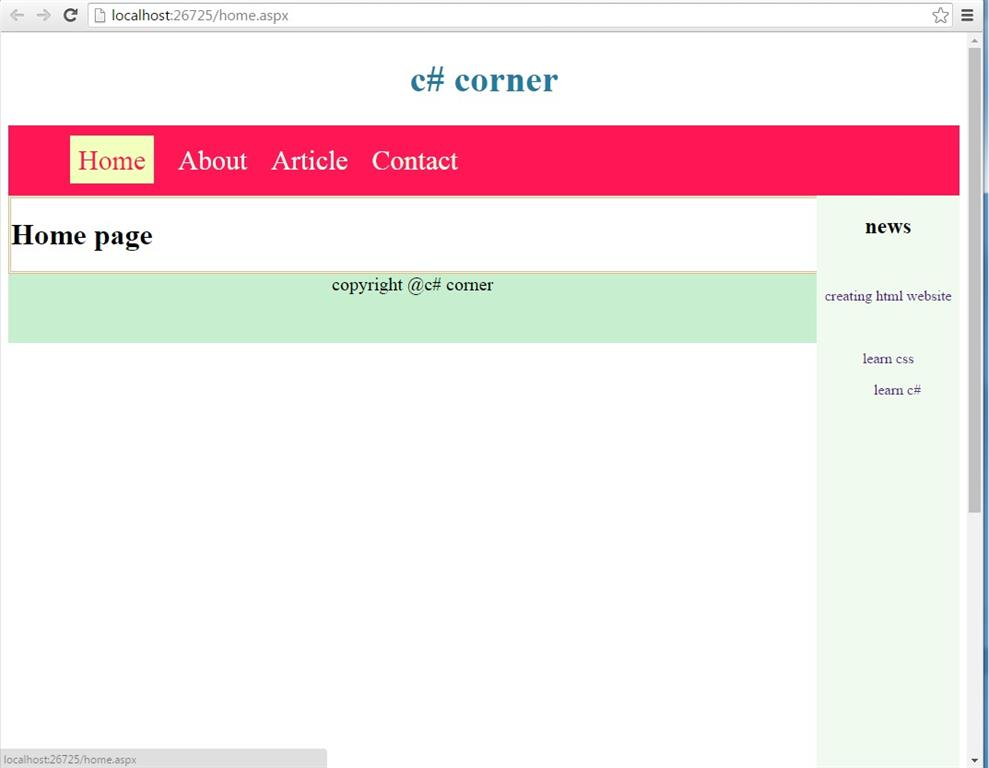
\includegraphics[width=0.85\linewidth]{img/a2}
	\caption{\textit{Table Instance}}
	\label{fig:create_table}
\end{figure}


\section{SELECT}
It is the most basic SQL query one can use for manipulating a database. The select command is used to select the data from the database and display it to the user.

\subsection{DISTINCT Keyword}
If we want to display certain field without any duplicates then we use the DISTINCT keyword along with the select command.
Example:
\begin{lstlisting}[language=sql]
	Select DISTINCT FName From Student;
\end{lstlisting}

\subsection{WHERE Clause}
If we need only certain records from the table then we use the where clause. Where clause acts as a Filtering mechanism. Under the Where section we need to specify certain conditions, only if those conditions are met the records will be extracted.
Syntax:
\begin{lstlisting}[language=sql]
	SELECT column1, column2, ...column N FROM table_name WHERE condition;
\end{lstlisting}
Example:
\begin{lstlisting}[language=sql]
	SELECT FName FROM Students WHERE City='Delhi';
\end{lstlisting}

\subsection{AND, OR, NOT Operators}
If we need to add two or more conditions in the where clause then we can use the above-mentioned operators. These keywords will add more complexity to the query.

\subsubsection{AND Operator}
This operator displays a record if all the conditions separated by AND are TRUE.
Syntax:
\begin{lstlisting}[language=sql]
	SELECT column1, column2, ...FROM table_name WHERE condition1 AND condition2 AND condition3 ...;
\end{lstlisting}
Example:
\begin{lstlisting}[language=sql]
	SELECT * FROM Student WHERE FName='John' AND Lname='Doe';
\end{lstlisting}

\subsubsection{OR Operator}
This operator displays a record if any of the conditions separated by OR is TRUE.
Syntax:
\begin{lstlisting}[language=sql]
	SELECT column1, column2, ... FROM table_name WHERE condition1 OR condition2 OR condition3 ...;
\end{lstlisting}
Example:
\begin{lstlisting}[language=sql]
	SELECT * FROM Student WHERE FName='John' OR Lname='Doe';
\end{lstlisting}

\subsubsection{NOT Operator}
This operator displays a record if the condition/conditions are NOT TRUE.
Syntax:
\begin{lstlisting}[language=sql]
	SELECT column1, column2, ...FROM table_name WHERE NOT condition;
\end{lstlisting}
Example:
\begin{lstlisting}[language=sql]
	SELECT * FROM Student WHERE NOT Lname='Doe';
\end{lstlisting}

\chapter{AGGREGATE Functions}
\section{Introduction}
An aggregate function is a function where the values of multiple rows are grouped together as input on certain criteria and a single value is returned. We often use aggregate functions with the GROUP BY and HAVING clauses of the SELECT statement.

Some of the Aggregate functions are COUNT, SUM, AVG, MIN, MAX.

\section{COUNT()}
This function returns the number of rows that match specified criteria.
Syntax:
\begin{lstlisting}[language=sql]
	SELECT COUNT(column_name) FROM table_name;
\end{lstlisting}
Example:
\begin{lstlisting}[language=sql]
	SELECT COUNT (studentID) FROM Student;
\end{lstlisting}

\section{AVG()}
This function returns the average value of a numeric column.
Syntax:
\begin{lstlisting}[language=sql]
	SELECT AVG(column_name) FROM table_name;
\end{lstlisting}
Example:
\begin{lstlisting}[language=sql]
	SELECT AVG(Marks) FROM Student;
\end{lstlisting}

\section{SUM()}
This function returns the total sum of a numeric column.
Syntax:
\begin{lstlisting}[language=sql]
	SELECT SUM(column_name) FROM table_name;
\end{lstlisting}
Example:
\begin{lstlisting}[language=sql]
	SELECT SUM(Marks)FROM Student;
\end{lstlisting}

\section{MIN()}
This function returns the smallest value of the selected column.
Syntax:
\begin{lstlisting}[language=sql]
	SELECT MIN(column_name)FROM table_name;
\end{lstlisting}
Example:
\begin{lstlisting}[language=sql]
	SELECT MIN(Marks) AS LeastMarks FROM Student;
\end{lstlisting}

\section{MAX()}
This function returns the largest value of the selected column.
Syntax:
\begin{lstlisting}[language=sql]
	SELECT MAX(column_name) FROM table_name;
\end{lstlisting}
Example:
\begin{lstlisting}[language=sql]
	SELECT MAX(Marks) AS HighestMarks FROM Student;
\end{lstlisting}


\chapter{Group By, Having, Order By}
\section{GROUP BY}
This functionality is used to arrange a similar type of data into a group. For instance, if the column in a table consists of similar data or value in different rows then we can use GROUP BY function to group the data.
Syntax:
\begin{lstlisting}[language=sql]
	SELECT column_name(s) FROM table_name WHERE condition GROUP BY column_name(s);
\end{lstlisting}
Example:
\begin{lstlisting}[language=sql]
	SELECT COUNT(StudentID), Fname FROM Student GROUP BY Fname;
\end{lstlisting}

\section{HAVING}
This clause is used to place conditions where we need to decide which group will be the part of final result-set. Also, we can not use the aggregate functions like SUM(), COUNT() etc. with WHERE clause. At such situation, we have to use HAVING condition.
Syntax:
\begin{lstlisting}[language=sql]
	SELECT column_name(s) FROM table_name WHERE condition GROUP BY column_name(s) HAVING condition;
\end{lstlisting}
Example:
\begin{lstlisting}[language=sql]
	SELECT Fname, SUM(Marks) FROM Student GROUP BY Fname HAVING SUM(Marks)>500;
\end{lstlisting}

\section{ORDER BY}
This keyword is used to sort the result-set in ascending or descending order. The ORDER BY keyword shall sort the records in ascending order by default. If we want to sort the records in descending order, use the DESC keyword.
Syntax:
\begin{lstlisting}[language=sql]
	SELECT column1, column2, ... FROM table_name ORDER BY column1, column2, ... ASC|DESC;
\end{lstlisting}
Example:
\begin{lstlisting}[language=sql]
	SELECT COUNT(StudentID), City FROM Student GROUP BY City ORDER BY COUNT(StudentID) DESC;
\end{lstlisting}

\chapter{NULL Values and Some more Operators}

\section{NULL Values}
In SQL we use the NULL term to represent a missing value. A NULL value in a table is a value appears to be blank. A field with a NULL value is a field with no value in SQL. Keep note that a NULL value is different than a zero value or a field that contains spaces. We have special keywords i.e, IS NULL and IS NOT NULL.

\subsection{IS NULL}
Syntax:
\begin{lstlisting}[language=sql]
	SELECT column_names FROM table_name WHERE column_name IS NULL;
\end{lstlisting}
Example:
\begin{lstlisting}[language=sql]
	Select Fname, Lname From Student Where Marks IS NULL;
\end{lstlisting}

\subsection{IS NOT NULL}
Syntax:
\begin{lstlisting}[language=sql]
	SELECT column_names FROM table_name WHERE column_name IS NOT NULL;
\end{lstlisting}
Example:
\begin{lstlisting}[language=sql]
	Select Fname, Lname From Student Where Marks IS NOT NULL;
\end{lstlisting}


\section{IN Operator}
IN operator is used to specify multiple values inside the WHERE clause. It acts as a short for multiple OR.
Syntax:
\begin{lstlisting}[language=sql]
	SELECT column_name(s) FROM table_name WHERE column_name IN (value1, value2, ...); 
\end{lstlisting}
Example:
\begin{lstlisting}[language=sql]
	SELECT StudentID, Fname, Lname FROM Student WHERE City IN ('Delhi', 'Goa', 'Pune','Bengaluru');
\end{lstlisting}

\section{BETWEEN Operator}
BETWEEN operator will select a particular value within the specified range. It is compulsory to add the beginning and the end value (Range).
Syntax:
\begin{lstlisting}[language=sql]
	SELECT column_name(s) FROM table_name WHERE column_name BETWEEN value1 AND value2;
\end{lstlisting}
Example:
\begin{lstlisting}[language=sql]
	SELECT StudentID, Fname, Lname FROM Student WHERE Marks BETWEEN 400 AND 500;
\end{lstlisting}

\section{UNION Operator}
UNION Syntax:
\begin{lstlisting}[language=sql]
	SELECT Column1, Column2, Column3, ..., ColumnN FROM Table1
	UNION
	SELECT Column1, Column2, Column3, ..., ColumnN FROM Table2;	
\end{lstlisting}
UNION ALL Syntax:
\begin{lstlisting}[language=sql]
	SELECT Column1, Column2, Column3, ..., ColumnN FROM Table1
	UNION ALL
	SELECT Column1, Column2, Column3, ..., ColumnN FROM Table2;
\end{lstlisting}


\section{INTERSECT Operator}
This clause used to combine two SELECT statements and return the intersection of the data-sets of both the SELECT statements.
Syntax:
\begin{lstlisting}[language=sql]
	SELECT Column1 , Column2 .... FROM TableName WHERE Condition
	INTERSECT
	SELECT Column1 , Column2 .... FROM TableName WHERE Condition;
\end{lstlisting}